\documentclass[journal, a4paper, twoside, romanappendices]{IEEEtran}
% !TEX root = ./report.tex

\usepackage{datetime}		%For \newdateformat
\usepackage{float}			%For forcing position of figures
\usepackage{listings}		%For code in document
\usepackage[usenames,%
dvipsnames]{xcolor}			%For the SkyBlue background color for lstlistings
\usepackage{todonotes}		%For \todo
\usepackage{tabularx}		%for tablecontents wrapping inside cell, instead of cell breaking page width.
\usepackage{enumerate}		%For getting different types of lists like a) II) and so forth.
\usepackage[utf8,%
utf8x]{inputenc}			%For norwegian letters and UTF8 encoding support
\usepackage{lastpage}		%For the command \pageref{lastpage}
\usepackage[colorlinks]{hyperref}		%For \url{}
\usepackage{pdfpages}		%For including pdfs
\usepackage{appendix}		%For appendix in article
\usepackage[nottoc,%
numbib]{tocbibind}			%For references in Table of Contents
\usepackage[english]{babel}	%For filltext in conjunction with blindtext
\usepackage{blindtext}		%For filltext (see comment for babel)
\usepackage{caption}		%For use of the \caption command inside minipage environment
\usepackage{standalone}		%For being able to inlclude project_description which has begin{document}
\usepackage{geometry}		%For scaling/setting margin size and so on
%\usepackage{svg}			%For includesvg command
%\usepackage{textgreek}	%Test

%\setsvg{svgpath = figures/}
%\setsvg{inkscape = inkscape -z -D}

\hypersetup{linkcolor=black}
\hypersetup{citecolor=black}
\hypersetup{urlcolor=black}

\newdateformat{CurMonth}{\monthname[\THEMONTH],~\THEYEAR}

\lstset{
	language=C++,				% choose the language of the code
	basicstyle=\tiny,			% the size of the fonts that are used for the code
	numbers=left,				% where to put the line-numbers
	numberstyle=\tiny,			% the size of the fonts that are used for the line-numbers
	stepnumber=1,				% the step between two line-numbers. If it is 1 each line will be numbered
	numbersep=5pt,				% how far the line-numbers are from the code
	backgroundcolor=\color{White},	% choose the background color. You must add \usepackage{color}
	showspaces=false,			% show spaces adding particular underscores
	showstringspaces=false,		% underline spaces within strings
	showtabs=false,				% show tabs within strings adding particular underscores
	frame=none,					% adds a frame around the code
	keywordstyle={},			% sets the graphical style of keywords in the language
	tabsize=4,					% sets default tabsize to 4 spaces
	captionpos=b,				% sets the caption-position to bottom
	breaklines=true,			% sets automatic line breaking
	breakatwhitespace=false,	% sets if automatic breaks should only happen at whitespace
	escapeinside={@}{@}			% if you want to add a comment within your code
}

\lstdefinestyle{customcpp}{
	frame=l,							%
	tabsize=2,							% sets default tabsize to 4 spaces
	language=C++,						%
	numbers=left,						% where to put the line-numbers
	stepnumber=1,						% the step between two line-numbers. If it is 1 each line will be numbered
	captionpos=b,						% sets the caption-position to bottom
	numbersep=5pt,						% how far the line-numbers are from the code
	showtabs=false,						% show tabs within strings adding particular underscores
	breaklines=true,					% sets automatic line breaking
	showspaces=false,					% show spaces adding particular underscores
	numberstyle=\tiny,					% the size of the fonts that are used for the line-numbers
	escapeinside={@}{@},				% if you want to add a comment within your code
	showstringspaces=false,				% underline spaces within strings
	xleftmargin=\parindent,				%
	breakatwhitespace=true,				% sets if automatic breaks should only happen at whitespace
	stringstyle=\color{Orange},			%
	identifierstyle=\color{Blue},		%
	backgroundcolor=\color{White},		% choose the background color. You must add \usepackage{color}
	belowcaptionskip=1\baselineskip,	%
	basicstyle=\footnotesize,			%
	commentstyle=\itshape\color{Brown},%
	keywordstyle=\bfseries\color{Green},% sets the graphical style of keywords in the language
}

\lstset{literate=
	{á}{{\'a}}1 {é}{{\'e}}1 {í}{{\'i}}1 {ó}{{\'o}}1 {ú}{{\'u}}1
	{Á}{{\'A}}1 {É}{{\'E}}1 {Í}{{\'I}}1 {Ó}{{\'O}}1 {Ú}{{\'U}}1
	{à}{{\`a}}1 {è}{{\'e}}1 {ì}{{\`i}}1 {ò}{{\`o}}1 {ù}{{\`u}}1
	{À}{{\`A}}1 {È}{{\'E}}1 {Ì}{{\`I}}1 {Ò}{{\`O}}1 {Ù}{{\`U}}1
	{ä}{{\"a}}1 {ë}{{\"e}}1 {ï}{{\"i}}1 {ö}{{\"o}}1 {ü}{{\"u}}1
	{Ä}{{\"A}}1 {Ë}{{\"E}}1 {Ï}{{\"I}}1 {Ö}{{\"O}}1 {Ü}{{\"U}}1
	{â}{{\^a}}1 {ê}{{\^e}}1 {î}{{\^i}}1 {ô}{{\^o}}1 {û}{{\^u}}1
	{Â}{{\^A}}1 {Ê}{{\^E}}1 {Î}{{\^I}}1 {Ô}{{\^O}}1 {Û}{{\^U}}1
	{œ}{{\oe}}1 {Œ}{{\OE}}1 {æ}{{\ae}}1 {Æ}{{\AE}}1 {ß}{{\ss}}1
	{ç}{{\c c}}1 {Ç}{{\c C}}1 {ø}{{\o}}1 {å}{{\r a}}1 {Å}{{\r A}}1
	{€}{{\EUR}}1 {£}{{\pounds}}1
}


\begin{document}

\title{When should one inline recursive functions?}
\author{Christian~Chavez}
\maketitle

\thanks{Nico~Reissmann, Magnus~Jahre, and Christian~Chavez are with the
Norwegian University of Science and Technology (NTNU).}


\begin{IEEEkeywords}
Function inlining, Jive, Compiler, 2015, NTNU
\end{IEEEkeywords}

\begin{abstract}

Lorem ipsum...

\end{abstract}

%% !TEX root = ./report.tex

\section{Dictionary}

\todo[inline]{Figure out the terms found in papers...}

\subsection{\textit{placeholder}}
\todo[inline]{Insert reference to ``GHC secrets'' -paper in subsection title above}

\begin{itemize}

	\item Section 1
\begin{itemize}

	\item ``inlining subsumes''
	\item ``lexical scopes''
	\item ``pure'' (\textit{language})
	\item ``explicitly typed'' (\textit{language})
	\item ``strictness analysis''
	\item ``\textit{let}-floating'' (\textit{Haskell})
	\item ``name capture''

\end{itemize}

	\item Section 2
\begin{itemize}

	\item ``\textit{$\beta$}-reduction''
	\item ``invariant'' (\textit{language artifact/variable/expression?})
	\item ``\textit{trivial-constructor-argument invariant}'' (\textit{Haskell?
})
	\item ``divergent computations''
	\item ``closure'' (\textit{scopes of functions?})
	\item ``lambda calculus''
	\item ``literals''
	\item ``primitive operators''

\end{itemize}

	\item Section 3
\begin{itemize}

	\item ``bound variable''
	\item ``recursive binding groups''
	\item ``strongly-connected components''
	\item ``one-shot lambdas''
	\item ``contravariantly''
	(\textit{(..) it appears contravariantly in its own definition.})
	\item ``ùntyped programs''
	\item ``pathological programs''
	\item ``static analysis''

\end{itemize}

	\item Section 4
\begin{itemize}

	\item ``hash-consing''

\end{itemize}

\end{itemize}

% !TEX root = ./report.tex

\section{Introduction}
\todo[inline]{Describe layout of paper. What does each section in turn discuss?}

\subsection{Problemsetting}

\todo[inline]{Re-state the assignment: Inlining -> Easy, what is it, benefits/drawbacks. \\
``This paper details the problems and benefits of inlining'' \\
Introduce Jive in a few sentences, say that it's further introduced in section
2.}

Inlining is a straight-forward technique used in code compilation, which
replaces the call of a function with the body of said function. Its benefits
include removal of function call overhead (1) and unveiling of additional
potential optimizations in the code (2). The drawbacks are potentially increased
code size (3), as well as longer execution times for the compilation of the
program (4).

The contribution of this paper is an inliner for the Jive backend
compiler\footnote{Detailed in Section \ref{background:jive}.}, detailing the
problems and benefits of inlining wrt. inlining in the Jive compiler. Jive is a
new backend compiler which works on intermediate representation (IR) code, and
performs the typically expected compiler techniques and optimizations on said IR
code with the help of a new type of graph; the regionalized value-state
dependency graph (RVSDG\footnote{Detailed in Section \ref{background:RVSDG}.}).

Further details of this assignment can be found in Appendix
\ref{app:projdesc}.

% !TEX root = ./report.tex

\clearpage
\section{The Regionalized Value State Dependence Graph}
\label{background:RVSDG}

The \textit{Regionalized Value State Dependence Graph}~\cite{RVSDG:HiPEACpaper}
(RVSDG) is a \textit{directed acyclic \nolinebreak{demand-based} dependence graph},
consisting of nodes representing computations and edges representing the
dependencies between nodes. Each node has inputs and outputs connected through
edges. The arity and order of inputs and outputs depend on the operation the
node represents, and need to match the operation.

Figure~\ref{fig:simple_node_RVSDG_ex} exemplifies how the C/C++ code on the left
can be represented as an RVSDG. The nodes in
Figure~\ref{fig:simple_node_RVSDG_ex} represent operations in a program, while
the edges between the nodes show the dependencies nodes have to each other, thus
giving the order of execution.

In all RVSDG examples depicted in this report, the order of inputs in a node
goes clockwise. The first input of a node is the one closest to the bottom left
corner of the node.

\begin{centering}
	\noindent\begin{minipage}{0.36\textwidth}
		\begin{CenteredBox}
		\begin{lstlisting}[label={lst:simple_node_RVSDG_ex},
style=minipage_customcpp, basicstyle=\fontsize{10}{1}]
x = (y*2) / (z+2);
		\end{lstlisting}
		\end{CenteredBox}
	\end{minipage}
	\noindent\begin{minipage}{0.55\textwidth}
		\captionsetup{type=figure}
		\includegraphics[width=\textwidth]{figures/svg/simple_node_RVSDG_ex}
	\end{minipage}
	\captionof{figure}{Example depicting an RVSDG subgraph representing the
arithmetic operations and their data dependence edges corresponding to the C/C++
on the left.}
	\label{fig:simple_node_RVSDG_ex}
\end{centering}

\subsection{Edges}

The RVSDG has data- and state- edges, representing data and state dependencies
operations have to each other, respectively. An example of data dependence edges
are the operands used in an addition, such as in
Figure~\ref{fig:simple_node_RVSDG_ex}.

State dependence edges are used to preserve the semantics of the program when
the program has \nolinebreak{side-effecting} operations. If there are no data dependencies
between operations, state dependence edges can give the needed order of
execution. Figure~\ref{fig:load_dependence_ex} illustrates the use of state
dependence edges, depicted as dotted edges.

\begin{centering}
	\noindent\begin{minipage}{0.36\textwidth}
		\begin{CenteredBox}
		\begin{lstlisting}[label={lst:load_dependence_ex},
style=minipage_customcpp, basicstyle=\fontsize{10}{1}]
*x += 7;
*y += 7;
		\end{lstlisting}
		\end{CenteredBox}
	\end{minipage}
	\noindent\begin{minipage}{0.55\textwidth}
		\captionsetup{type=figure}
		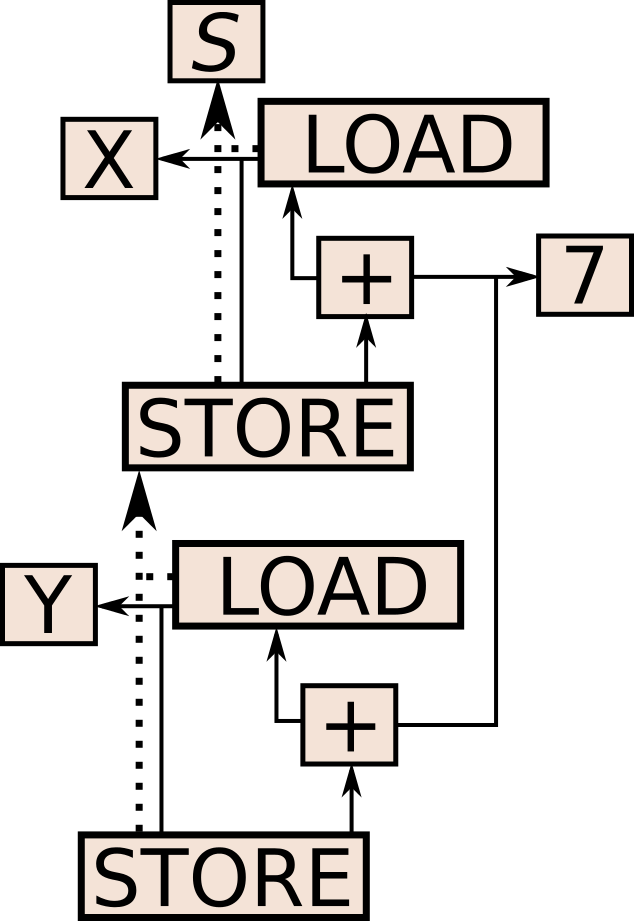
\includegraphics[width=\textwidth]{figures/svg/load_store_state_dependence_ex}
	\end{minipage}
	\captionof{figure}{Figure of an RVSDG subgraph exemplifying the need for and
use of state dependence edges. The RVSDG represents the equivalent of the C/C++
on the left. The \textit{S}-node in the figure supplies the needed state edge
for \lstinline!x!'s \textit{load}- and \textit{store}-nodes.}
	\label{fig:load_dependence_ex}
\end{centering}

\subsection{Nodes}

The RVSDG has two kinds of nodes: simple and complex nodes.

\subsubsection{Simple Nodes}

Simple nodes are used to represent primitive operations, such as addition and
subtraction. Figure~\ref{fig:simple_node_RVSDG_ex} is an example of an RVSDG
containing only simple nodes.

One simple node of special interest for this report is the \applyNode . An
\applyNode~represents the call site of a function. The first input argument of
an \applyNode~is the function the \applyNode~invokes. The remaining inputs are
the arguments to this function. Likewise, its results are the results of the
invocation of its function. Order and arity of inputs and outputs need to match
the arguments and results of the function, respectively.

\subsubsection{Complex Nodes}

Complex nodes contain one or more RVSDG subgraphs, which is why they are also
referred to as \textit{regions}. Differing from the simple nodes with their
contained subgraph, complex nodes may besides the normal inputs and outputs,
also have internal inputs and outputs. Figure~\ref{fig:complex_node_mapping_ex}
shows which inputs/outputs are the external ones, and which are the internal
ones. Figure~\ref{fig:complex_node_mapping_ex} also illustrates how the values
of the external inputs are mapped to the internal outputs of each subregion, and
vica versa with each sub-region's internal inputs being mapped to the external
outputs.

\begin{figure}[H]
	\centering
	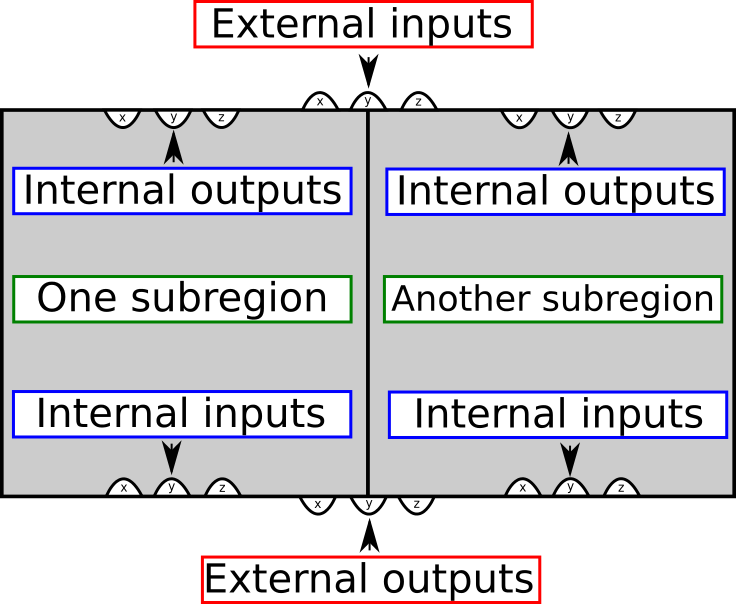
\includegraphics[width=0.7\textwidth]{figures/svg/complex_node_mapping_ex}
	\caption{An example of a complex node, showing which inputs/outputs
are external/internal, and how they can have multiple subregions.}
	\label{fig:complex_node_mapping_ex}
\end{figure}

As Figure~\ref{fig:complex_node_mapping_ex} also shows, some complex nodes may
also have multiple \textit{subregions}. If a complex node has more than one
subregion, the arity and order of all the internal inputs/outputs must match
between all subregions, as well as match the arity and order of the external
inputs/outputs of the complex node.

The complex nodes of an RVSDG relevant for this report are as follows:

\begin{itemize}

\item \textbf{$\gamma$-nodes: N-way statements}

\textit{$\gamma$-nodes} represent conditional statements. Each $\gamma$-node has
a predicate as first input. All other edges passing as inputs to the
$\gamma$-node are edges its subregions depend upon. Each subregion represents
one case. All subregions must have the same order and arity of internal inputs
and outputs, even if the subgraph in each region does not depend on all of the
internal outputs.

A $\gamma$-node is equivalent to a \textit{switch-case} without \nolinebreak{fall-through} in
C/C++. Each case of the switch statement corresponds to a subregion of the
$\gamma$-node. Hence, a simple \textit{if-statement} with no \nolinebreak{else-clause} can be
represented by a $\gamma$-node with two subregions. The true subregion contains
the RVSDG subgraph that represents the body of the if-statement, whereas the
false subregion of the $\gamma$-node simply routes all inputs through. See
Figure~\ref{fig:simple_if} for an example of a $\gamma$-node.

\begin{centering}
	\noindent\begin{minipage}{0.36\textwidth}
		\begin{CenteredBox}
		\begin{lstlisting}[label={lst:simple_if}, style=minipage_customcpp,
basicstyle=\fontsize{10}{1}]
if((z+2) != 0 ){
	x = (y*2) / (z+2);
}
		\end{lstlisting}
		\end{CenteredBox}
	\end{minipage}
	\noindent\begin{minipage}{0.55\textwidth}
		\captionsetup{type=figure}
		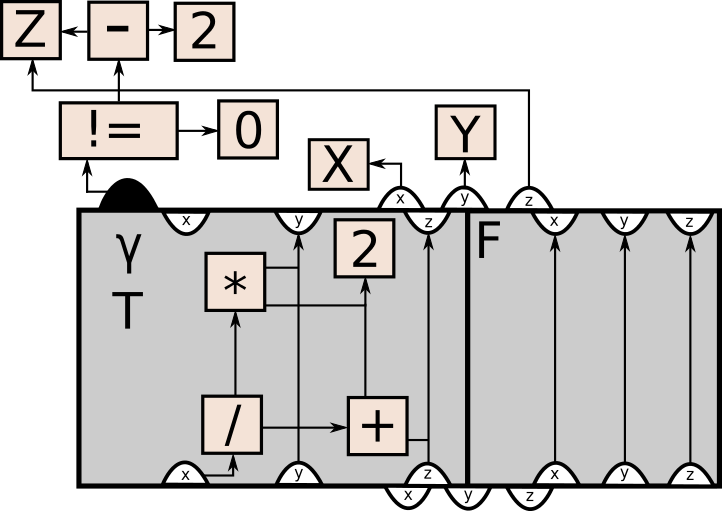
\includegraphics[width=\textwidth]{figures/svg/simple_if_example}
	\end{minipage}
	\captionof{figure}{An example of an RVSDG subgraph containing a
$\gamma$-node, representing an if-statement, corresponding to the C/C++ on the
left.}
	\label{fig:simple_if}
\end{centering}

\item \textbf{$\theta$-nodes: Tail-controlled loops}

\textit{$\theta$-nodes} represent \nolinebreak{tail-controlled} loops. As with
$\gamma$-nodes, its inputs (and outputs) are all the dependencies needed for the
RVSDG subgraph in its subregion.

The first time the body of the loop is executed, the external inputs are
mapped to the internal outputs, as Figure~\ref{fig:factorial_loop_ex}
exemplifies. This enables the complex node's contained in the RVSDG subgraph to
execute with the values given as external inputs to the $\theta$-node.

However, inside the $\theta$-node there is an extra first internal input, which
is the predicate of the \nolinebreak{tail-controlled} loop. If this predicate evaluates to
true, the rest of the internal inputs of the $\theta$-node are mapped to their
corresponding internal outputs. This enables the iterative behavior of an RVSDG
$\theta$-node. Thus, the operations represented by its contained RVSDG subgraph
are executed as a \nolinebreak{tail-controlled} loop. Finally, when the predicate evaluates to
false, the internal inputs are mapped to the external outputs of the
$\theta$-node instead of the internal outputs.

A $\theta$-node is equivalent to a \textit{do-while} loop in C/C++, as shown in
Figure~\ref{fig:factorial_loop_ex}.

\begin{centering}
	\noindent\begin{minipage}{0.36\textwidth}
		\begin{CenteredBox}
		\begin{lstlisting}[style=minipage_customcpp,
label={lst:fig:factorial_loop_ex}, basicstyle=\fontsize{10}{1}]
uint32_t i = 0;
uint64_t r = 1;
do {
	i += 1;
	r *= i;
} while(i < n);
		\end{lstlisting}
		\end{CenteredBox}
	\end{minipage}
	\noindent\begin{minipage}{0.55\textwidth}
		\captionsetup{type=figure}
		\includegraphics[width=\textwidth]{figures/svg/iterative_factorial_ex}
	\end{minipage}
	\captionof{figure}{An RVSDG subgraph depicted on the right, on the right,
containing a $\theta$-node representing the C/C++ do-while loop on the left.}
	\label{fig:factorial_loop_ex}
\end{centering}

A \textit{head-controlled} loop can be represented by putting a $\theta$-node
inside the subregion representing the true clause of a $\gamma$-node.
Additionally, both the $\gamma$-node's first input and the first internal input
of the $\theta$-node need to share the same predicate. Finally, the
$\gamma$-node's subregion representing the false clause cannot contain nodes.

\item \textbf{$\lambda$-nodes: Functions}

\textit{$\lambda$-nodes} represent functions. A $\lambda$-node contains an RVSDG
subgraph representing the body of a function. The internal inputs of a
$\lambda$-node represents the results of the function. Respectively, its
internal outputs represent the arguments of the function. While $\lambda$-nodes
don't have any external inputs, their external output are what give the
\applyNode s their first input, enabling them to invoke the function represented
by the $\lambda$-node.

The arity and order of a $\lambda$-node's internal inputs and outputs must match
the arity and order of the external inputs and outputs of all connected
\applyNode s.

Hence, when an \applyNode~connected with a $\lambda$-node is executed, the
external inputs of the \applyNode~are mapped to the internal outputs of the
$\lambda$-node, before the $\lambda$-node is invoked.

Likewise the internal inputs of the $\lambda$-node are mapped to the external
outputs of the \applyNode~when the operations of the $\lambda$-node have been
executed. See Figure~\ref{fig:iterative_factorial_func_ex} for an example of a
$\lambda$-node.

\begin{centering}
	\noindent\begin{minipage}{0.37\textwidth}
		\begin{CenteredBox}
		\begin{lstlisting}[label={lst:iterative_factorial_func_ex},
style=minipage_customcpp, basicstyle=\fontsize{10}{1}]
uint64_t fac(uint32_t n){
	uint32_t i = 0;
	uint64_t r = 1;
	do{
		i += 1;
		r *= i;
	} while(i < n);
	return r;
}
		\end{lstlisting}
		\end{CenteredBox}
	\end{minipage}
	\noindent\begin{minipage}{0.55\textwidth}
		\captionsetup{type=figure}
		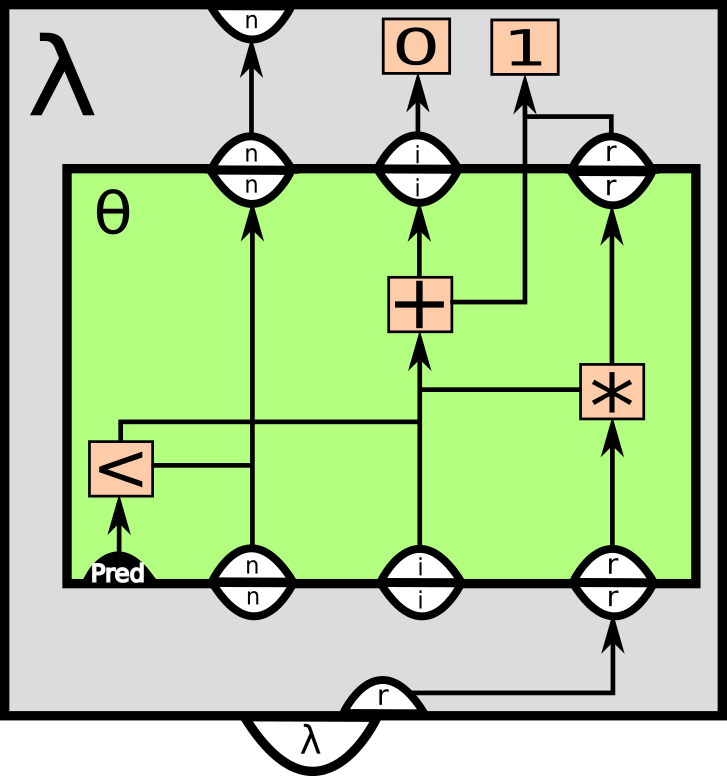
\includegraphics[width=\textwidth]{figures/svg/iterative_factorial_func_ex}
	\end{minipage}
	\captionof{figure}{Example of an RVSDG subgraph depicted on the right,
containing a $\lambda$-node representing the C/C++ function on the left.}
	\label{fig:iterative_factorial_func_ex}
\end{centering}

\item \textbf{$\phi$-regions: Recursive environments}

\textit{$\phi$-regions} represent recursive environments. They contain at least
one recursive $\lambda$-node. Like the $\lambda$-node, they have no external
inputs. However, the internal outputs of the $\phi$-region represent the links
utilized by the \applyNode s contained within to connect with the respective
$\lambda$-nodes.

The internal inputs of a $\phi$-region receive the function invocation links
from the $\lambda$-nodes contained within. The internal inputs map to the
external outputs, thus enabling \applyNode s outside of the recursive
environment to connect with the $\lambda$-nodes, as depicted in
Figure~\ref{fig:recursive_factorial_func_ex}.

\begin{centering}
	\noindent\begin{minipage}{0.37\textwidth}
		\begin{CenteredBox}
		\begin{lstlisting}[label={lst:recursive_factorial_func_ex},
style=minipage_customcpp, basicstyle=\fontsize{10}{1}]
uint64_t fac(uint32_t n){
	uint64_t r = 1;
	if(n > 1){
		r = n*fac(n-1);
	}
	return r;
}
		\end{lstlisting}
		\end{CenteredBox}
	\end{minipage}
	\noindent\begin{minipage}{0.55\textwidth}
		\captionsetup{type=figure}
		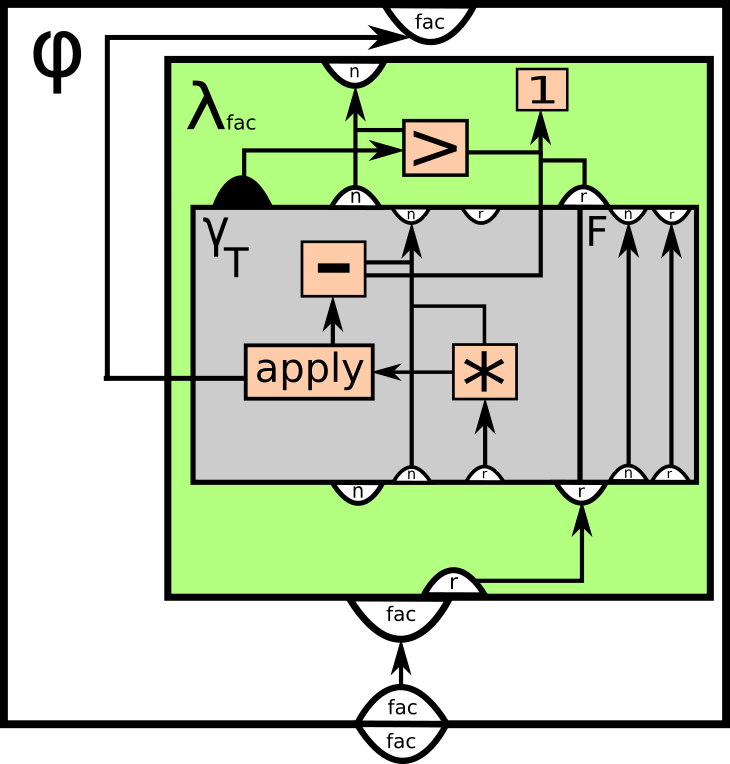
\includegraphics[width=\textwidth]{figures/svg/recursive_factorial_func_ex}
	\end{minipage}
	\captionof{figure}{Example of an RVSDG subgraph depicted on the right,
containing a $\phi$-region containing a representation of the recursive C/C++
function on the left.}
	\label{fig:recursive_factorial_func_ex}
\end{centering}

\end{itemize}

% !TEX root = ./report.tex

\section{Scheme}

% !TEX root = ./report.tex

\clearpage
\section{Methodology}

\todo[inline]{Need an introduction here, no?}

\subsection{Heuristics}

The heuristics used in the project described by this report can be divided into
to main subcategories: the heuristics of which \textit{apply}-nodes to look at
first, and the heuristics of whether or not to inline a single
\textit{apply}-node.

\subsubsection{Ordering of the \textit{apply}-node}

\subsubsection{The decision of inlining each \textit{apply}-node}

% !TEX root = ./report.tex

\clearpage
\section{Results}
\label{sec:res}

In this section, we first profile the Benchmarks introduced in
Section~\ref{sec:methodology}. Then, we profile the \applyNode s in the
Benchmark Suite specifically, before we explain the reasoning behind the
placeholder values we decided upon for the CNF we used in our testing.

Thereafter we show and discuss the results of our testing. We test with both the
top-down and bottom-up traversals discussed in
Section~\ref{sub:scheme:ordering_apply_nodes}. Some focus is put on the status
of Jive, and how its status may have affected our test results.

All averages discussedi in this section are linear averages.

\subsection{Profiling SPEC2006 and its functions}
\label{sub:res:profiling}

To decide upon the placeholder values for the the CNF introduced in
Section~\ref{sub:meth:cnf}, we profiled the SPEC2006 Benchmarks for the
following properties among others:

First and foremost, while a higher node count may still result in faster
execution in some cases, minimizing the amount of operations in a programs'
RVSDG was one of our main motivations behind deciding the placeholder values of
the CNF.

\begin{centering}
	\noindent\begin{minipage}{\textwidth}
		\captionsetup{type=figure}
		\hspace{-1em}
		\includegraphics[width=\textwidth]{figures/gnuplot/avg_node_count_pre_inlining}
	\end{minipage}
	\captionof{figure}{Histogram showing the average amount nodes present in
each SPEC2006 Benchmark. The y-axis is broken up due the two benchmark's
\textit{ h264ref} and \textit{lbm}'s big difference in average node count.}
	\label{fig:benchmarks_avg_nc_pre_inlining}
\end{centering}

Figure~\ref{fig:benchmarks_avg_nc_pre_inlining} shows the averaged
node count for each of the SPEC2006 Benchmarks used. We use
Figure~\ref{fig:benchmarks_avg_nc_pre_inlining} as our baseline, to which we
compare the results of our testing in Sections~\ref{sub:res:inlining_top_down}
and \ref{sub:res:inlining_bottom_up}.

The reason behind \textit{lbm}'s high node count average is caused by one of
\textit{lbm}'s files which contains functions that fill/modify large
\lstinline!IO_FILE!s with content. \textit{h264ref} also stands out, though not
as much as \textit{lbm}. It stands out due to its low average of nodes per file.
It does so because it only has one file which made it past the requirements
listed in Section~\ref{sub:meth:SPEC2006_files}, specifically requirement 3, and
the majority of this file consists of two leaf functions.

This observation raises the obvious point that by profiling the functions in the
benchmarks, we can observe how many of the functions are exported, seeing as
Jive is unable to link the program files at compile time. This would give us an
upper bound for how many functions we can remove through \textit{Dead Code
Elimination} (DCE). Figure~\ref{fig:avg_lambda_count_pre} shows us how many
functions there are on average in each Benchmark, and how big of an average of
these are exported.

\begin{centering}
	\noindent\begin{minipage}{\textwidth}
		\captionsetup{type=figure}
		\hspace{-1em}
		\includegraphics[width=\textwidth]{figures/gnuplot/avg_lambda_count_pre}
	\end{minipage}
	\captionof{figure}{Histogram showing that there is a small number of
functions we can hope to eliminate through DCE. The left bar shows the average
count of $\lambda$-nodes per benchmark, while the right bar shows the average
count of exported $\lambda$-nodes in the same benchmark.}
	\label{fig:avg_lambda_count_pre}
\end{centering}

One of the IC most used in our final CNF form is \textit{Node Count} (NC).
Hence, knowing what NC functions have on average in our test files is helpful.
Figure~\ref{fig:benchmarks_avg_nc_in_lambda_per_file} depicts this in a scatter
plot.

\begin{centering}
	\noindent\begin{minipage}{\textwidth}
		\captionsetup{type=figure}
		\hspace{-1em}
		\includegraphics[width=\textwidth]{figures/gnuplot/avg_nc_in_lambdas_pre}
	\end{minipage}
	\captionof{figure}{Scatter plot showing the spread of average amount of
nodes contained within each function per file in the Benchmarks Suite. The files
are grouped by Benchmark along the horizontal axis.}
	\label{fig:benchmarks_avg_nc_in_lambda_per_file}
\end{centering}

The spread of data points in
Figure~\ref{fig:benchmarks_avg_nc_in_lambda_per_file} tells us that while there
are some functions like the aforementioned of \textit{gcc}, the majority of them
contain less than 100 nodes. Which conforms well with the stipulation that most
applications majority of nodes are leaf nodes, which generally contain few
operations. This makes it somewhat easier for us to decide what limits NC should
present with regards to inlining, since we can see that a majority would be
inlined if we inlined all functions satisfying \lstinline|NC < 200|.

The histogram in Figure~\ref{fig:phis_and_lambdas_in_phis} tells us that there
are no recursive environments containing more than one function in the
Benchmarks tested. In other words, that all the recursive functions are
\nolinebreak{self-recursive}. As such, we did not get to test our algorithm
detailed in Section~\ref{sub:scheme:inlining_recur_apply_nodes} with the
SPEC2006 Benchmark Suite, but in our own testing we did confirm that it
permitted us to safely inline \textit{some} functions inside a recursive
environment containing multiple functions.

\begin{centering}
	\noindent\begin{minipage}{\textwidth}
		\captionsetup{type=figure}
		\hspace{-1em}
		\includegraphics[width=\textwidth]{figures/gnuplot/avg_phis_and_lambdas_in_phis}
	\end{minipage}
	\captionof{figure}{Histogram showing the average amount of $\phi$-regions
per benchmark with the left bar. The left bar shows the average amount of
$\lambda$-nodes inside each $\phi$-region present in a benchmark.}
	\label{fig:phis_and_lambdas_in_phis}
\end{centering}

Another property of functions of interest to us is the average amount of call
sites contained within functions. This property gives us an idea as to the
proportion of how many leaf nodes there are, containing no function calls, in a
benchmark, in addition to the proportion of functions with $X$ amount of call
sites on average.

Figure~\ref{fig:benchmarks_avg_cin_lambda_per_file} shows us that on average the
balance between functions with no call sites, and functions with, is not sharply
skewed one way or the other. We do have some outliers, like the aforementioned
files from \textit{gcc}, but one can safely say from the plot that a majority of
the functions have less than two hundred call sites contained within.

The histogram in Figure~\ref{fig:benchmarks_avg_cin_lambda_per_file} shows that
beneath the average of two hundred call sites in function mark on the y-axis,
there is a slight predominance for functions to have about one hundred or less.
These observations are helpful in giving us upper bounds for how many functions
could potentially be inlined by this IC.

\begin{centering}
	\noindent\begin{minipage}{\textwidth}
		\captionsetup{type=figure}
		\hspace{-1em}
		\includegraphics[width=\textwidth]{figures/gnuplot/avg_cin_pre_count}
	\end{minipage}
	\captionof{figure}{Scatter plot showing the spread of average amount of call
sites contained in functions per file in the Benchmarks Suite. The files are
grouped by Benchmark along the horizontal axis.}
	\label{fig:benchmarks_avg_cin_lambda_per_file}
\end{centering}

The final function property we profile is the amount of call sites invoking a
function. As the first clause of our CNF form states, if the function is not
exported, and there's only one invocation of the function, it is an easy
decision to inline.

However, by graphing the spread of how many call sites each files' functions
have on average, it gives us an idea of how many more functions could
potentially be inlined if just some of its invocations are inlined.
Figure~\ref{fig:benchmarks_avg_scc_lambda_per_file} shows us a scatter plot of
this data across all the test files used in the Benchmark Suite. The few
functions in the bottom right corner of the plot are functions which have no
call sites inside the same file, but are exported, meaning that if the
benchmark's program files were statically linked during compilation, there would
be no functions with zero static call sites.

What the data in Figure~\ref{fig:benchmarks_avg_scc_lambda_per_file} tells us,
is that the majority of functions are called just once. Seeing as Jive has not
statically linked the files in the benchmark during the creation of the RVSDG,
this is understandable. If Jive was able to build the RVSDG with statically
linked files, our suspicion is that the range of the vertical axis, and spread
data along it, would most likely grow.

\begin{centering}
	\noindent\begin{minipage}{\textwidth}
		\captionsetup{type=figure}
		\hspace{-1em}
		\includegraphics[width=\textwidth]{figures/gnuplot/avg_scc_pre_count}
	\end{minipage}
	\captionof{figure}{Scatter plot showing the spread of average Static Call
Counts for functions per file in the Benchmarks Suite. The files are grouped by
Benchmark along the horizontal axis.}
	\label{fig:benchmarks_avg_scc_lambda_per_file}
\end{centering}

However, as the data stands, we can see that if a function is not exported, and
two of its invocations are inlined, there is a decent chance of applying DCE on
the functions.

\subsection{Profiling SPEC2006's \applyNode s}
\label{sub:res:ic_profiling}

In our profiling, the data we are most interested relates to the \applyNode s in
the benchmarks. First we check in
Figure~\ref{fig:statically_known_applies_vs_all_applies} how many \applyNode s
each benchmark contains, and which of these we can potentially inline. Our
definition of \textit{statically known} apply-\textit{nodes}, is as follows: if
the $\lambda$-node invoked is directly connected to the \applyNode~in the RVSDG,
or resides within a $\phi$-region, which in turn is connected directly to the
\applyNode , it is statically known.

We cannot inline \applyNode s which are not statically known, and since Jive is
unable to link files at compile time, there is conceivably large portion of
\applyNode s not statically known. If Jive had been able to create and process
RVSDGs composed of linked object files, instead of just disparate files, the
proportion of statically known \applyNode s may have been higher.
Figure~\ref{fig:statically_known_applies_vs_all_applies} shows the )
average count of \applyNode s per SPEC2006 Benchmark in the left bar, and the
) average count of the statically known in the right bar.

\begin{centering}
	\noindent\begin{minipage}{\textwidth}
		\captionsetup{type=figure}
		\hspace{-1em}
		\includegraphics[width=\textwidth]{figures/gnuplot/avg_static_and_not_apply_nodes}
	\end{minipage}
	\captionof{figure}{Histogram showing the average count of \applyNode s (left
bar), and the average count of statically known \applyNode s (right bar), per
benchmark.}
	\label{fig:statically_known_applies_vs_all_applies}
\end{centering}

As Figure~\ref{fig:statically_known_applies_vs_all_applies} also shows, there
are only two benchmarks with more than ten statically known \applyNode s and
$\lambda$-nodes each. This time \textit{gcc} is the one with numbers high above
the rest with regards to the $\lambda$-node average, but what is shown is that
\textit{gcc}'s \applyNode~average also stands above the rest. Further
investigation reveals that there is one lone file inside the Benchmark which has
over six thousand \applyNode s and almost eight hundred $\lambda$-nodes. This
particular file contains almost only functions, many of which invoke multiple
others, thereby achieving these numbers.

\begin{centering}
	\noindent\begin{minipage}{\textwidth}
		\captionsetup{type=figure}
		\hspace{-1em}
		\includegraphics[width=\textwidth]{figures/gnuplot/avg_pc_cpc_pre_count}
	\end{minipage}
	\captionof{figure}{Scatter plot showing the spread of average Parameter
Count per file in the Benchmarks (plus signs), and the spread of average
Constant Parameter Count (depicted by tilted plus signs). The files are grouped
by Benchmark along the horizontal axis.}
	\label{fig:benchmarks_avg_pc_cpc}
\end{centering}

The data spread in Figure~\ref{fig:benchmarks_avg_pc_cpc} shows that there are
few function calls with up to six parameters, some of which have up to five
constant parameters in the invocation. The region of average parameter counts is
most dense in the area between $1.5$ and $2.5$ on the vertical axis. To avoid
inlining the majority of function calls, the lower limit of constant parameters
needed should be above two. Thus we avoid code size explosion by hindering
function invocations with only one or two constant parameters, while we permit
function invocations with more to become inlined.

Finally, one of the most important properties of a call site with regards to
inlining is the amount of nested loops it resides within.
Figure~\ref{fig:benchmarks_avg_lnd_per_file} plots the average LND count of the
call sites in a Benchmark Suite test file. The scatter plot in
Figure~\ref{fig:benchmarks_avg_lnd_per_file} tells us that there are no call
sites (\applyNode s) residing within more than two nested loops. While research
shows that most of a programs' execution time is spent inside of loops, it is
useful to have an idea of the proportion of call sites within one, two, or zero
loops. If the CNF clause checking for LND of our CNFs final form sets the
threshold at three or higher, the clause would be useless, since there are no
call sites satisfying the requirement present in the test files.

\begin{centering}
	\noindent\begin{minipage}{\textwidth}
		\captionsetup{type=figure}
		\hspace{-1em}
		\includegraphics[width=\textwidth]{figures/gnuplot/avg_lnd_pre_count}
	\end{minipage}
	\captionof{figure}{Scatter plot showing the spread of average Loop Nesting
Depth for call sites per file in the Benchmarks Suite. The files are grouped by
Benchmark along the horizontal axis.}
	\label{fig:benchmarks_avg_lnd_per_file}
\end{centering}

\subsection{Final CNF}
\label{sub:res:final_cnf}

With the observations made from the profiling data, and some testing to find the
optimum values with regards to average node count size in the benchmarks, the
following values were used for our test results:

\begin{centering}
\lstinline!(EXP == false && SCC = 1) || NC < 25 || CIN < 3 ||! \\
\lstinline!(NC < 200 && CPC > 2) || (NC < 200 && LND > 0)! \\
\end{centering}

\subsection{Inlining results: top-down traversal}
\label{sub:res:inlining_top_down}

Since Jive is not able to produce executable code, we are unable to test the
timing of the RVSDGs our inliner has been executed on. Hence, as mentioned in
Section~\ref{sub:res:profiling}, our motivation has been to reduce the amount of
operations. This because we interpret the NC to be generally representative of
the time it would have taken to execute the optimized code.

Figure~\ref{fig:res:topdown_post_pre_nc_benchmarks} shows a histogram where the
averaged NC per benchmark is represented before and after the inliner has been
executed. While we repeat that these results must be taken with the proverbial
grain of salt due to Jive's inability to statically link the files of the
benchmarks, we do hope that they are somewhat representative of how the effects
of our inliner.

\begin{centering}
	\noindent\begin{minipage}{\textwidth}
		\captionsetup{type=figure}
		\hspace{-1em}
		\includegraphics[width=\textwidth]{figures/gnuplot/top_down_avg_nc_pre_post_benchmarks}
	\end{minipage}
	\captionof{figure}{Histogram showing the average NC per SPEC2006
Benchmark before (left bar), and after (right bar) inlining.}
	\label{fig:res:topdown_post_pre_nc_benchmarks}
\end{centering}

Figure~\ref{fig:res:topdown_wc_scatterplot} shows the spread of how much time
the inliner needs for processing the files in from the Benchmark Suite. Again,
the results are somewhat skewed due to Jive's status. Jive does not have all of
the common compiler techniques implemented either. Optimization techniques such
as auto vectorization and alias analysis are lacking in their entirety, and what
optimizations it does have are not completely bug-free.

\begin{centering}
	\noindent\begin{minipage}{\textwidth}
		\captionsetup{type=figure}
		\hspace{-1em}
		\includegraphics[width=\textwidth]{figures/gnuplot/top_down_wc_scatterplot}
	\end{minipage}
	\captionof{figure}{Scatterplot showing the spread of the time it takes in
(wall clock ms.) to execute the inliner per .c file tested in a top-down
traversal order.}
	\label{fig:res:topdown_wc_scatterplot}
\end{centering}

However, with the exception of the few outliers, we see that the majority of
test files were executed in under one second. As to the outliers needing up
towards 80 seconds to execute, due to Jive's status as under development, it is
difficult to determine for sure whether the majority of the time is spent in the
traversal of call sites, or in the necessary functions offered by
Jive\footnote{Discussed further in Section~\ref{sub:conclusion:summary}.}.

Table~\ref{sub:res:top_down_table} summarizes the NC results per SPEC2006
Benchmark pre- and post-inlining, giving a bit more detail and summarizing the
effects across all the files in the Benchmark Suite. The weighted average of
post-inlining NC divided by pre-inlining NC across all benchmarks give us a
$6.79\%$ average reduction in NC after executing our inliner.

\begin{table}[h!]
	\centering
	\caption{Top-down post- and pre-inlining Node Count averages per SPEC2006 Benchmark}
	\label{sub:res:top_down_table}
	\begin{tabular}{|c|c|c|c|c|c|}
	\hline
	\multicolumn{1}{|l|}{{\bf \rotatebox{75}{ SPEC2006 Benchmarks } }} & \multicolumn{1}{l|}{{\bf \rotatebox{75}{ Average Node Count Pre-Inlining } }} & \multicolumn{1}{l|}{{\bf \rotatebox{75}{ Average Node Count Post-Inlining } }} & \multicolumn{1}{l|}{{\bf \rotatebox{75}{ \% Difference in Node Count } }} & \multicolumn{1}{l|}{{\bf \rotatebox{75}{ \# Files per Benchmark } }} & \multicolumn{1}{l|}{{\bf \rotatebox{75}{ \% of files total in Benchmark } }} \\ \hline
	{\it bzip2 } & 1481.250 & 494.750 & 33.401\% & 4 & 1.254 \\ \hline
	{\it gcc } & 1771.660 & 1368.319 & 77.234\% & 47 & 14.734 \\ \hline
	{\it gobmk } & 2152.158 & 2001.421 & 92.996\% & 19 & 5.956 \\ \hline
	{\it gromacs } & 1838.741 & 1700.941 & 92.506\% & 85 & 26.646 \\ \hline
	{\it h264ref } & 61.000 & 61.000 & 100.000\% & 1 & 0.313 \\ \hline
	{\it hmmer } & 1537.667 & 1482.222 & 96.394\% & 45 & 14.107 \\ \hline
	{\it lbm } & 5612.000 & 5627.500 & 100.276\% & 2 & 0.627 \\ \hline
	{\it libquantum } & 297.000 & 321.750 & 108.333\% & 8 & 2.508 \\ \hline
	{\it mcf } & 437.222 & 438.667 & 100.330\% & 9 & 2.821 \\ \hline
	{\it milc } & 439.231 & 441.019 & 100.407\% & 52 & 16.301 \\ \hline
	{\it perlbench } & 850.857 & 872.571 & 102.552\% & 7 & 2.194 \\ \hline
	{\it sjeng } & 1133.125 & 1058.375 & 93.403\% & 8 & 2.508 \\ \hline
	{\it sphinx3 } & 1182.406 & 1199.875 & 101.477\% & 32 & 10.031 \\ \hline
	\end{tabular}
\end{table}


\FloatBarrier

\subsection{Inlining results: bottom-up traversal}
\label{sub:res:inlining_bottom_up}

The testing for the bottom-up ordering was performed identically as the top-down
orderings tests. Thus we will display the same table and figures, but with new
data and our guesses as to the difference between the two. The one notable
exception between the two being that one of the test files in the \textit{hmmer}
benchmark was unable to complete the execution within the allotted 120 seconds.

\begin{centering}
	\noindent\begin{minipage}{\textwidth}
		\captionsetup{type=figure}
		\hspace{-1em}
		\includegraphics[width=\textwidth]{figures/gnuplot/bottom_up_avg_nc_pre_post_benchmarks}
	\end{minipage}
	\captionof{figure}{Histogram showing the average NC per SPEC2006
Benchmark before (left bar), and after (right bar) inlining.}
	\label{fig:res:bottomup_post_pre_nc_benchmarks}
\end{centering}

Figure~\ref{fig:res:bottomup_post_pre_nc_benchmarks} shows a very similar trend
to Figure~\ref{fig:res:topdown_post_pre_nc_benchmarks}. So from NC alone there
does not seem to be much difference between the averaged NCs per benchmark.

The spread in Figure~\ref{fig:res:bottomup_wc_scatterplot} shows that while the
spread along the vertical axis does not go as high in the bottom-up traversal as
for the top-down traversal, there are more test files requiring more than half a
second to execute with the inliner. While the top-down ordering takes an average
$1279.213$ ms. to execute, the bottom up ordering takes $1576.028$ ms.

Table~\ref{sub:res:bottom_up_table} summarizes the same results from the
SPEC2006 Benchmark Suite as Table~\ref{sub:res:top_down_table}, though with
bottom-up traversal instead. However, what is worth noticing, is that the
weighted average of post-inlining NC divided by pre-inlining NC across all
benchmarks gives a $6.98\%$ average reduction in NC after executing our
inliner.

\begin{centering}
	\noindent\begin{minipage}{\textwidth}
		\captionsetup{type=figure}
		\hspace{-1em}
		\includegraphics[width=\textwidth]{figures/gnuplot/bottom_up_wc_scatterplot}
	\end{minipage}
	\captionof{figure}{Scatterplot showing the spread of the time it takes in
(wall clock ms.) to execute the inliner per .c file tested in a bottom-up
traversal order.}
	\label{fig:res:bottomup_wc_scatterplot}
\end{centering}

The discrepancy between the top-down and bottom-up traversals averages of NC and
execution time may be explained by the following: Top-down traversal inlines
leaf nodes first into their callees, while bottom-up inlines the first functions
in nested functions calls first. While some research suggests that the majority
of execution is sometimes spent in leaf nodes, the call sites in side of nested
loops, which we also seek to optimize, will be the ones most likely to be
inlined first with the bottom-up ordering. This could account for the increased
reduction of operations, since as more operations are collected closer to the
root function\footnote{Comparable to C/C++'s \lstinline!main()!.}, the chances
for applying DCE increases.

The timing can also be accounted for, since leaf nodes tend to have a lesser NC,
the cost for Jive to inline a leaf node is very likely smaller than inlining a
function from the the top of the nested call stack into its predecessor. Thus,
for optimal results, a balance could perhaps be found between the two.


\begin{table}[h]
	\centering
	\caption{Bottom-up post- and pre-inlining Node Count averages per SPEC2006 Benchmark}
	\label{sub:res:bottom_up_table}
	\begin{tabular}{|c|c|c|c|c|c|}
	\hline
	\multicolumn{1}{|l|}{{\bf \rotatebox{75}{ SPEC2006 Benchmarks } }} & \multicolumn{1}{l|}{{\bf \rotatebox{75}{ Average Node Count Pre-Inlining } }} & \multicolumn{1}{l|}{{\bf \rotatebox{75}{ Average Node Count Post-Inlining } }} & \multicolumn{1}{l|}{{\bf \rotatebox{75}{ \% Difference in Node Count } }} & \multicolumn{1}{l|}{{\bf \rotatebox{75}{ \# Files per Benchmark } }} & \multicolumn{1}{l|}{{\bf \rotatebox{75}{ \% of files total in Benchmark } }} \\ \hline
	{\it bzip2 } & 1481.250 & 494.750 & 33.401\% & 4 & 1.258 \\ \hline
	{\it gcc } & 1771.660 & 1351.766 & 76.299\% & 47 & 14.780 \\ \hline
	{\it gobmk } & 2152.158 & 1974.842 & 91.761\% & 19 & 5.975 \\ \hline
	{\it gromacs } & 1838.741 & 1690.400 & 91.932\% & 85 & 26.730 \\ \hline
	{\it h264ref } & 61.000 & 61.000 & 100.000\% & 1 & 0.314 \\ \hline
	{\it hmmer } & 1555.455 & 1523.886 & 97.970\% & 44 & 13.836 \\ \hline
	{\it lbm } & 5612.000 & 5627.500 & 100.276\% & 2 & 0.629 \\ \hline
	{\it libquantum } & 297.000 & 325.375 & 109.554\% & 8 & 2.516 \\ \hline
	{\it mcf } & 437.222 & 438.667 & 100.330\% & 9 & 2.830 \\ \hline
	{\it milc } & 439.231 & 440.635 & 100.320\% & 52 & 16.352 \\ \hline
	{\it perlbench } & 850.857 & 872.571 & 102.552\% & 7 & 2.201 \\ \hline
	{\it sjeng } & 1133.125 & 1077.875 & 95.124\% & 8 & 2.516 \\ \hline
	{\it sphinx3 } & 1182.406 & 1188.656 & 100.529\% & 32 & 10.063 \\ \hline
	\end{tabular}
\end{table}

\FloatBarrier

% !TEX root = ./report.tex

\clearpage
\section{Discussion}

\section{Conclusion}

\subsection{Further Work}


\bibliography{bibliography}
\bibliographystyle{plain}

\end{document}
